\documentclass{beamer}
\usepackage[utf8]{inputenc}
\usepackage{subfig}
\usepackage{utopia} %font utopia imported
\usepackage{arabtex}
\usepackage{utf8}
\usepackage{amsmath}
\usepackage{amssymb}
\usepackage{amsthm}
\setcode{utf8}
\usetheme{Madrid}
\usecolortheme{default}

% This block of code defines the information to appear in the
% title page

\title[EMIR ] %optional
{IR drop and Electromigration}

\subtitle{Errors Can Break Your ASIC!}

\author[Ahmed Abdelazeem] % (optional)
{Ahmed Abdelazeem}
%{A.~B.~Arthur\inst{1} \and J.~Doe\inst{2}}

\institute[ZU] % (optional)
{
	Faculty of Engineering\\
	Zagazig University
}
%{
	%	\inst{1}%
	%	Faculty of Engineering\\
	%	Zagazig University
	%	\and
	%	\inst{2}%
	%	Faculty of Chemistry\\
	%	Very Famous University
	%}

\date[ZU 2023] % (optional)
{RTL2GDSII Flow, February 2022}

%\logo{
\includegraphics[height=1.5cm]{lion-logo.png}}

%End of title page configuration block
%------------------------------------------------------------

%------------------------------------------------------------
%The next block of commands puts the table of contents at the
%beginning of each section and highlights the current section:

\AtBeginSection[]
{
	\begin{frame}
		\frametitle{Table of Contents}
		\tableofcontents[currentsection]
	\end{frame}
}
%------------------------------------------------------------


\begin{document}
	
	%The next statement creates the title page.
	\frame{\titlepage}
	
	
	%---------------------------------------------------------
	%This block of code is for the table of contents after
	%the title page
	\begin{frame}
		\frametitle{Table of Contents}
		\tableofcontents
	\end{frame}
	%---------------------------------------------------------
	
	
	\section{Voltage (IR) Drop and Ground Bounce}
	
	%---------------------------------------------------------
	%Changing visivility of the text
	\begin{frame}
		\frametitle{Introduction}
		\begin{itemize}
			\item \textbf{IR drop:} Voltage drops caused by current flowing from the power source through the
			resistive power network to the on-chip devices is called IR drop.
			\item \textbf{Ground bounce:} Voltage spikes caused by current flowing from on-chip devices though the
			resistive ground network to the ground pins (or bumps)
			\item IR drop and ground bounce combine to impact silicon performance.
			
		\end{itemize}
		\begin{center}
		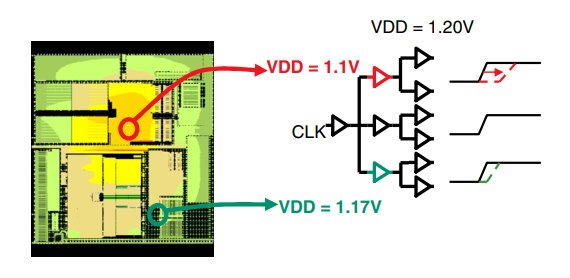
\includegraphics[width=0.8\textwidth]{IR1} 
		\end{center}
		


	\end{frame}
	
	%------------------------------------------------
	
	\begin{frame}
		\frametitle{IR Drop Impacts on Setup and Hold Time}
		\begin{itemize}
			\item In the case where the IR drop occurs within the signal path, the signal is
			slowed, potentially causing setup time violations for this signal path
		\end{itemize}
		\begin{center}
			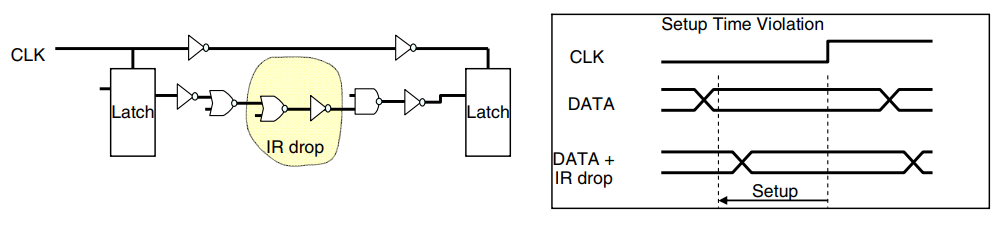
\includegraphics[width= 0.8\textwidth]{IR2}
		\end{center}
				\begin{itemize}
			\item In the case where IR drop occurs on a clock buffer, the clock signal beyond
			this buffer is slowed, potentially causing hold time violations for all signals
			clocked by this clock branch.
		\end{itemize}
		\begin{center}
			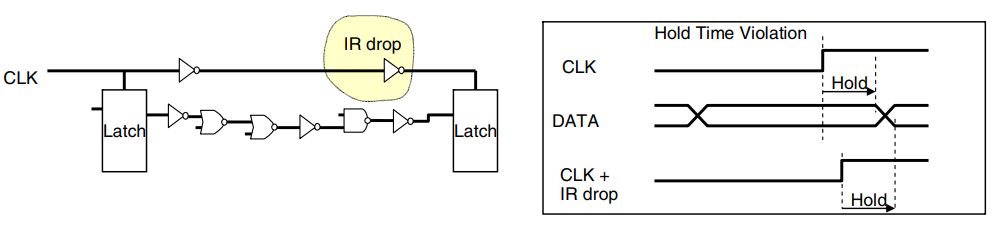
\includegraphics[width= 0.8\textwidth]{IR3}
		\end{center}
		
	\end{frame}
	%---------------------------------------------------------
	%Highlighting text
	\begin{frame}
		\frametitle{How Does a Power Rail IR Drop Occur?}
	\begin{center}
		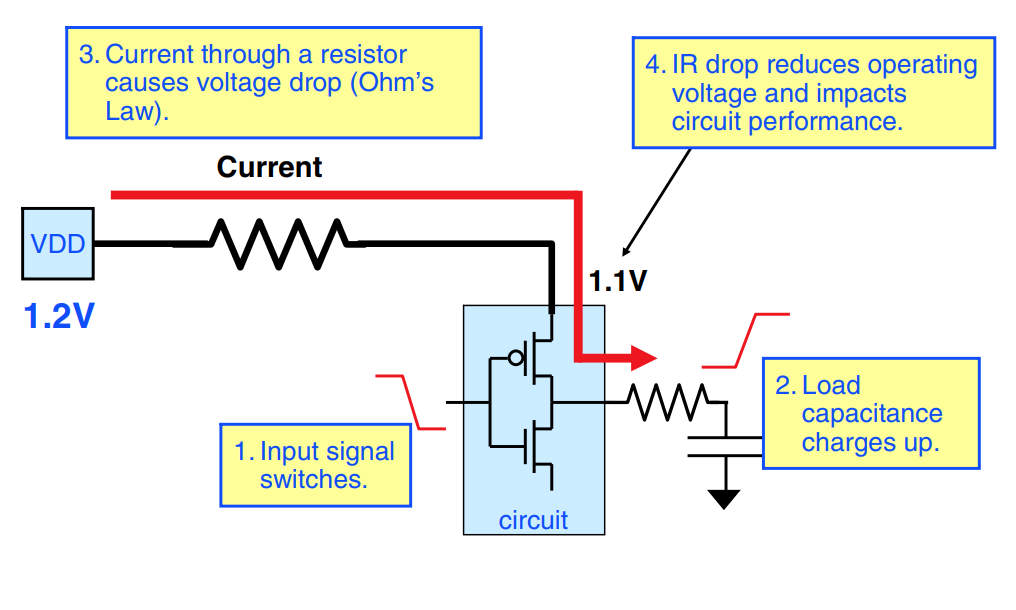
\includegraphics[width= 1\textwidth]{IR4}
	\end{center}
	\end{frame}	
	%---------------------------------------------------
	\begin{frame}
		\frametitle{IR Drop Occur}
		\begin{itemize}
			\item The power supply (VDD and VSS) in a chip is uniformly distributed through the metal rails and stripes which is called Power Delivery Network (PDN) or power grid.
			\item Each metal layers used in PDN has finite resistivity.
			\item When current flow through the power delivery network, a part of the applied voltage will be dropped in PDN as per the Ohm’s law
			\item The amount of voltage drop will be V = I.R, which is called the IR drop. 
			\item If the resistivity of metal wire is high or the amount of current following through the power net is high, A significant amount of voltage may be dropped in the power delivery network which will cause a lesser amount of voltage available to the standard cells than the actual amount of voltage applied.
		\end{itemize}
		
	\end{frame}
	
	\begin{frame}
		\frametitle{IR Continue}
		\begin{itemize}
			\item If V1 voltage is applied at the power port and current I is following in a particular net which has total resistance R, then the voltage available (V2) to the other end for the standard cell will be
				\begin{equation}
					V2 = V1 – I.R
				\end{equation}  
			\item Standard cells or macros sometimes do not get the minimum operating voltage which is required to operate them due to IR drop in power delivery network even the application of sufficient voltage in the power port. 
			\item Voltage drop in the power delivery network before reaching the standard cells is called IR drop. 
			\item This drop may cause the \textcolor{red} {poor performance} of the chip due to the increase of delay of standard cells and may cause the \textcolor{red} {functional failure} of the chip due to setup/hold timing violation. 
		\end{itemize}
	\end{frame}
	
	\begin{frame}
		\frametitle{Types of IR drop}
		\begin{block}{There are two types of IR drop in the ASIC design:}
			\begin{itemize}
				\item Static IR drop
				\item Dynamic IR drop
			\end{itemize}
		\end{block}
	\begin{itemize}
		\item Static IR drop is the voltage drop in the power delivery network (PDN) when there are no inputs switching means the circuit is in the static stage. 
		\item dynamic IR drop is the voltage drop in the power delivery network when the inputs are continuously switching means the circuit is in a functional state. Dynamic IR drop will depend on the switching rate of instance.
		\item When the inputs are switching continuously, more current would flow in the instances and also in PDN. So there will be more IR drop in the PDN. Therefore dynamic IR drop is more than the static IR drop.
	\end{itemize}		
	\end{frame}
	\begin{frame}
		\frametitle{Static vs. Dynamic IR Drop Analysis}
		\begin{center}
			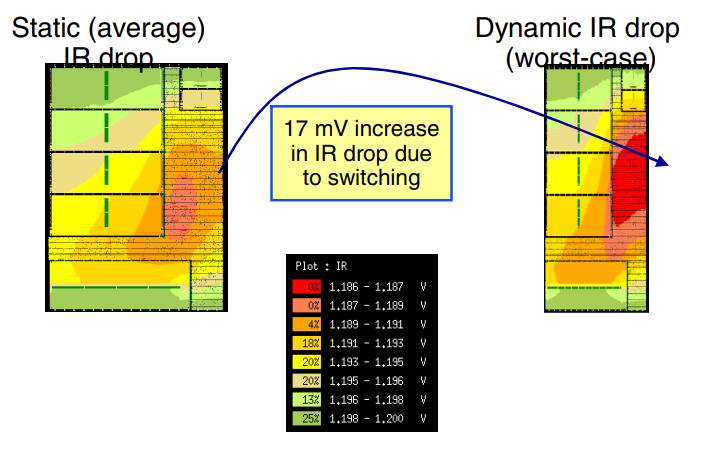
\includegraphics[width=\textwidth]{IR4_}
		\end{center}
		
	\end{frame}
	%-----------------------------------------------
	\begin{frame}
		\frametitle{Example Colors for IR Drop}
			\begin{center}
				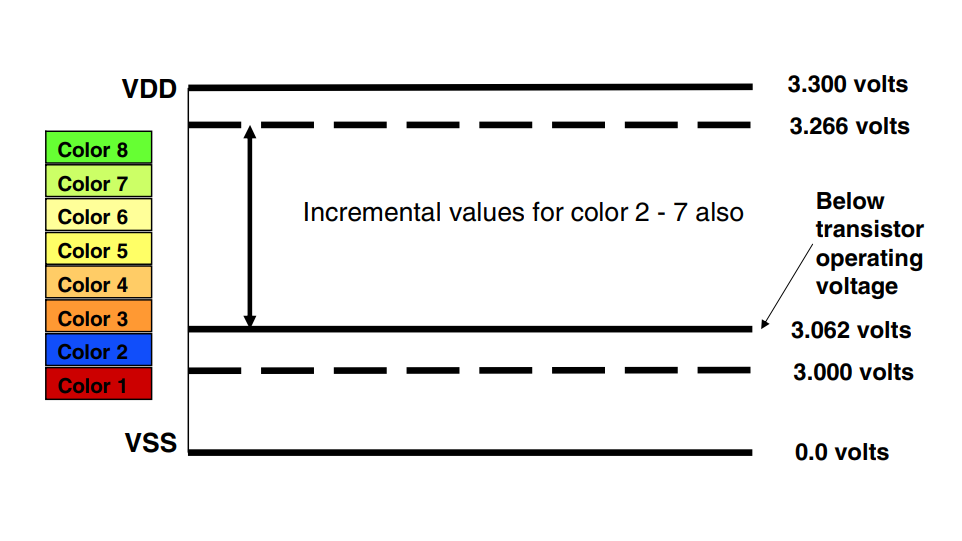
\includegraphics[width=\textwidth]{IR5}
			\end{center}
	\end{frame}	
		\begin{frame}
		\frametitle{IR Drop Example for Chip}
		\begin{center}
			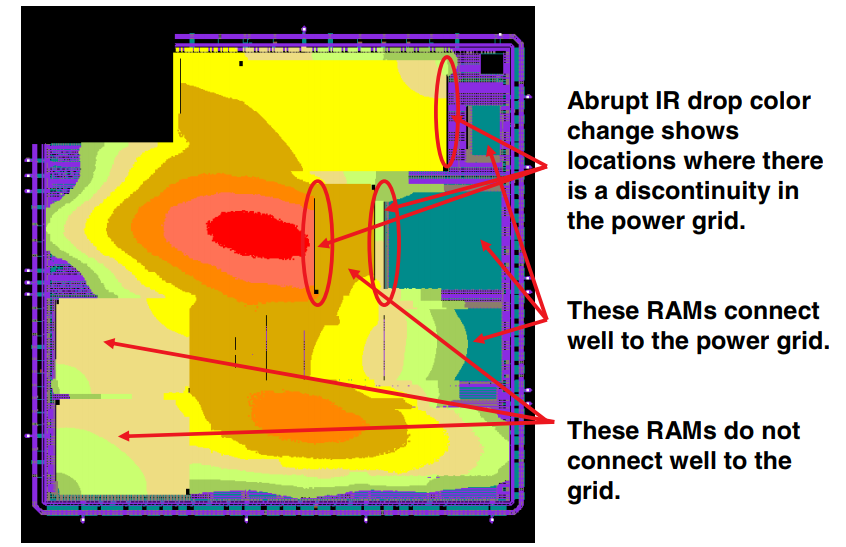
\includegraphics[width=\textwidth]{IR6}
		\end{center}
	\end{frame}	
	\begin{frame}
		\frametitle{Reasons for IR drop:)}
		IR drop could occur due to various reasons but some main reasons are as bellow.
		\begin{itemize}
			\item Poor design of power delivery network (lesser metal width and more separation in the power stripes)
			\item inadequate via in power delivery network 
			\item Inadequate number of decap cells availability
			\item High cell density and high switching in a particular region
			\item High impedance of the power delivery network
			\item Rush current 
			\item Insufficient number of voltage sources 
			\item High RC value of the metal layer used to create the power delivery network
		\end{itemize}
	\end{frame}
	
	\begin{frame}
	\frametitle{Method of Reducing Dynamic IR Drop}
		\begin{center}
			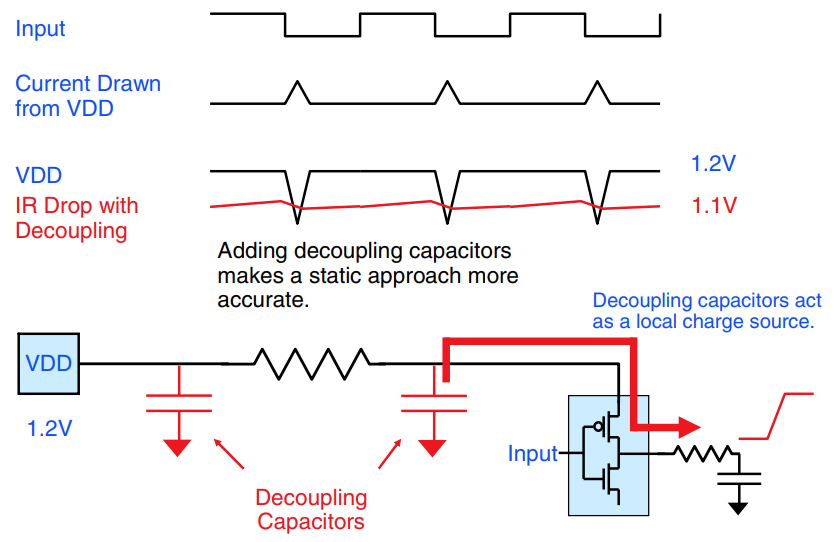
\includegraphics[width=\textwidth]{solu}
		\end{center}
	\end{frame}
	\begin{frame}
	\frametitle{Method of Reducing Static IR Drop}
	\begin{columns}
		\column{0.6\textwidth}
		\begin{itemize}
			\item The red area means a voltage drop of more than 10\% of the nominal supply voltage. The solution is to use wider power stripes or use more metal on higher levels.
			\item Additional power stripes are added to the design and are marked in cyan and magenta.
			\item This IR drop plot is made after an increase of the number of power stripes.
			\item This plot shows a very low voltage drop, which is required for a functional chip.
		\end{itemize}
		
		\column{0.6\textwidth}
		\begin{center}
			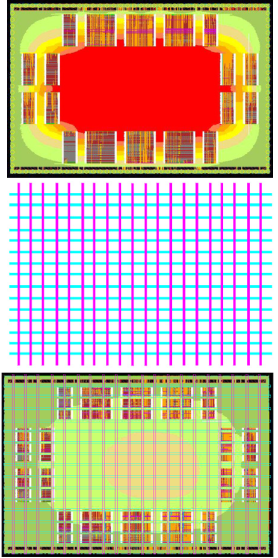
\includegraphics[width=0.5\textwidth]{solu2}
		\end{center}
	\end{columns}
	\end{frame}
	
	\begin{frame}
		\frametitle{Methods to improve IR drop}
		\begin{block}{Methods to improve static IR drop}
			\begin{itemize}
				\item We can go for higher layers if available
				\item Increase the width of the straps.
				\item Increase the number of wires.
				\item Check if any via is missing then add more via.
			\end{itemize}
		\end{block}
				\begin{block}{Methods to improve dynamic IR drop}
			\begin{itemize}
				\item Use de-cap cells.
				\item Increase the number of straps
			\end{itemize}
		\end{block}
		\begin{alertblock}{Tools used for IR drop analysis}
		\begin{itemize}
			\item RedHawk of Ansys.
			\item Voltus of Cadence Design System.
		\end{itemize}
		\end{alertblock}
	\end{frame}
	
	%------------------------------------------
	\section{Electromigration}
	\begin{frame}
		\frametitle{What is Electromigration?}
		\begin{block}{Definition}
			is the gradual displacement of metal atoms in a semiconductor. It happens when the current density is high enough to cause the drift of metal ions in the direction of the electron flow.
		\end{block}
		\begin{center}
			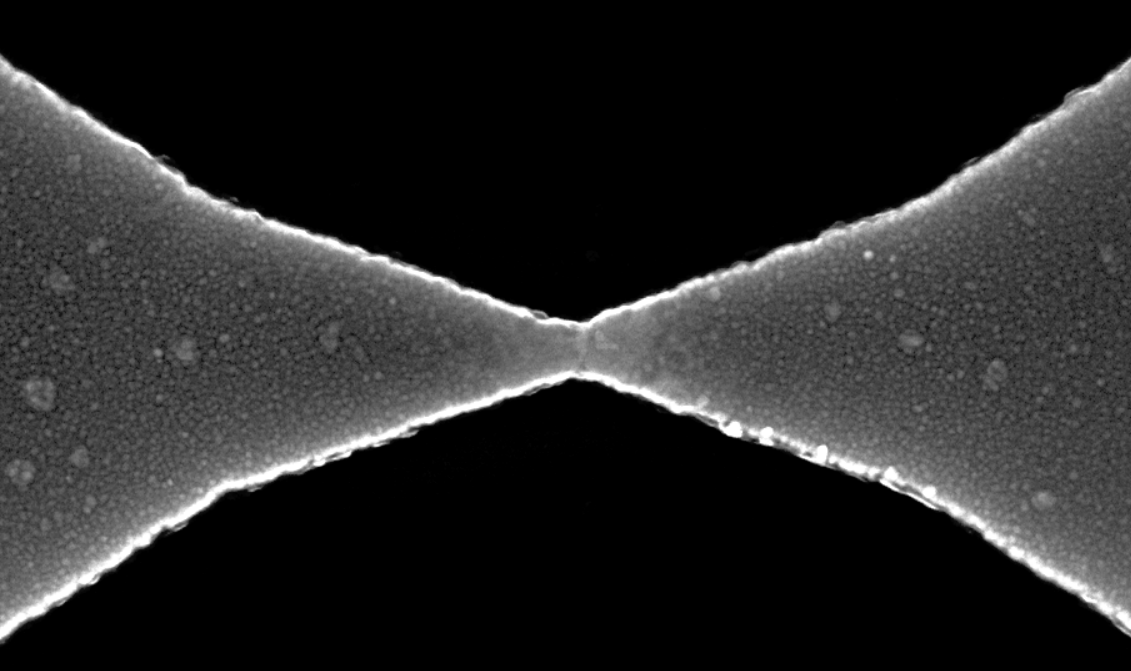
\includegraphics[width=0.7\textwidth]{EM_1}
		\end{center}
	\end{frame}
	\begin{frame}
		\frametitle{What is Electromigration?}
		Electromigration is a wear-out mechanism of metal wires.
		\newline
		\begin{itemize}
			\item Metal atoms migrate over a period of time, causing open circuits,
			shorts circuits, or unacceptable increases in resistance.
			\item There are two main causes of electromigration failure:
				\begin{enumerate}
					\item High (DC) current densities
					\item Joule heating, which is caused by high alternating currents
				\end{enumerate}
			\item These wear-out mechanisms can take extended periods of time
		\end{itemize}
	\begin{center}
		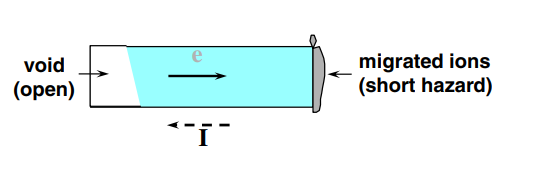
\includegraphics[width=\textwidth]{EM1}
	\end{center}
	\end{frame}	
	
	\begin{frame}
		\frametitle{Causes of Electromigration}
			\begin{itemize}
				\item Electromigration is mechanical failure in the wire caused by frequently varying
				thermal conditions.
				\item As pulses go through the wire, the power dissipated by the wire causes it to
				heat above oxide temperature
				\item The difference in the thermal constants between the oxide and the wire
				causes mechanical stress, and the wire can eventually fail resulting in chip
				failure in the field.
			\end{itemize}
	
\begin{center}
	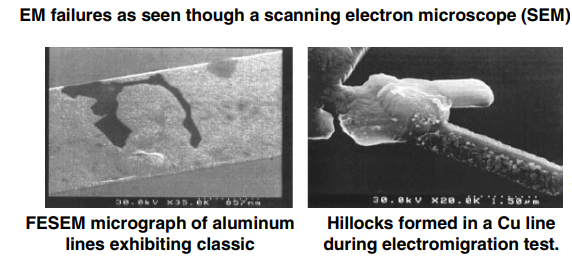
\includegraphics[width=0.7\textwidth]{em2}
\end{center}
	\end{frame}
	
	%-----------------------------------------------
	\begin{frame}
		\frametitle{Electromigration Damages}

	\begin{alertblock}{Effects of EM}
		\begin{itemize}
			\item Depletion of atoms (Voids): Slow reduction of connectivity; Interconnect failure
			\item Deposition of atoms (Hillocks): Shorts
		\end{itemize}
	\end{alertblock}
	\begin{center}
		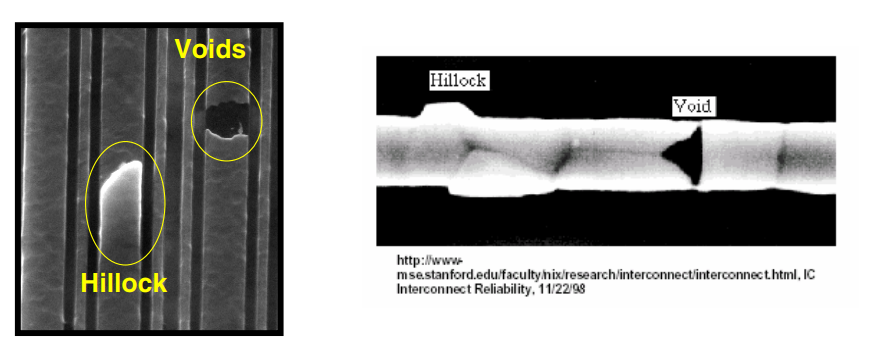
\includegraphics[width=0.8\textwidth]{em3}
	\end{center}
\end{frame}
	
	\begin{frame}
		\frametitle{High (DC) Current Densities}
		\begin{itemize}
			\item Physical migration of metal atoms due to “electron wind” can
			eventually create a break in a wire.
			\begin{itemize}
				\item (MTTF) is an indication of the life span of an integrated circuit. MTTF is calculated using Black’s equation as bellow.
			\begin{equation}
					MTTF = \frac{A}{J^n} exp(\frac{Ea}{KT})
				\end{equation}
			\item Current density must not exceed specification
			\item Specified as  \({mA}/~\mathrm{\text\textmu m}\)  wire width (e.g., \(1~\mathrm{mA/ \text\textmu m}\)) or mA per via cut
			\end{itemize}

			\item EM occurs both in signal (AC=bidirectional) and power wires
			(DC = unidirectional)
			\begin{itemize}
				\item Much worse for DC than AC; DC occurs inside cells and in power buses
			\end{itemize}
		\end{itemize}

	\end{frame}
	%-----------------------------------------------
	\begin{frame}
		\frametitle{Example: Current Density}
		\begin{center}
			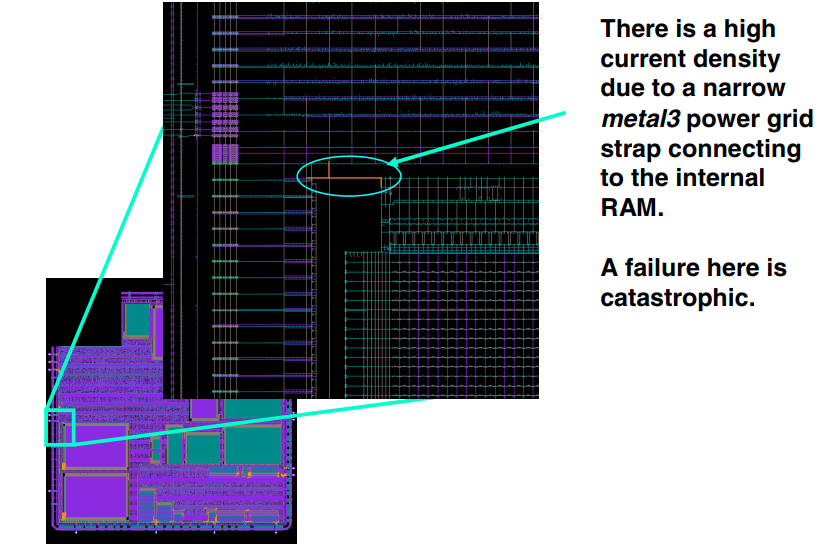
\includegraphics[width=\textheight]{em4}
		\end{center}

	\end{frame}	
	
	\begin{frame}
		\frametitle{Reasons of Electromigration}
		\begin{alertblock}{Reasons of EM Violation:}
			\begin{itemize}
				\item High Fanout Net(Multiple fanout cells switch simultaneously, draws larger current from driver)
				\item Higher Driver strength Cells (delivers large current unnecessarily, heating up the wire)
				\item Higher Frequency (quick tarnsitions)
				\item Narrow Metal Width.
				\item Metal slotting (resulting into narrower widths)
				\item Long Nets (because of larger resistance, higher localized temperature)
			\end{itemize}
		\end{alertblock}
	\end{frame}	
\begin{frame}
	\frametitle{Prevention techniques for  EM:}
	During the physical design, the following techniques could be used to prevent the EM issue.
	
	
	\begin{block}{Solutions of EM Violation:}
		\begin{itemize}
			
			\item Decrease Drive's drive Strength.
			\item Insert Buffer on long nets.
			\item Increase the width of wire
			\item Adding more vias (Multi-Cut Vias)
			\item Break the fanout (have lessar fanout)
			\item Switch the net to higher metal layers.
		\end{itemize}
	\end{block}
\end{frame}
	%------------------------------------------------
	
	\section{Other related Issues}	
	\begin{frame}
		\frametitle{What Is Joule Heating?}
		Wire Self-Heat (WSH)
		\begin{itemize}
			\item May also be called signal wire electromigration, or Joule heating, since it is related to the
			power that is dissipated into the interconnect.
			\item  WSH is the rise in temperature due to the electron movement within a conductor.
			\item  Depends on metal composition, signal frequency, wire sizes, slew rates, and amount of
			capacitance driven
			\item Self-heating = More EM
			\begin{itemize}
				\item Since SH increases temperature, self-heating on a metal line can aggravate EM effects.
				\item SH on a line can also increase EM effects on neighboring lines.
			\end{itemize}	
			\item Because self-heating contributes to electromigration, failures are typically labeled as EM, not SH.
		\end{itemize}
		\begin{center}
			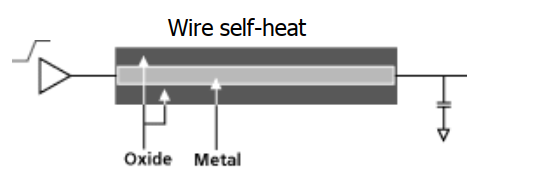
\includegraphics[width=0.5\textwidth]{joules}
		\end{center}
	\end{frame}
	\begin{frame}
		\frametitle{Hot Electron Effect (Short Channel Effect)}
	\begin{itemize}
		\item Caused by extremely high electric fields between source and drain
		\begin{itemize}
			\item Occurs when voltages are not scaled as fast as dimensions
		\end{itemize}	
		\item Electrons pick up speed in the channel
		\item Fastest electrons damage the oxide and interface near the drain
		\item Transistor threshold and mobility change over the life of the part, i.e.,
		threshold eventually moves to a point where the device no longer meets
		specifications
	\end{itemize}
	\begin{center}
	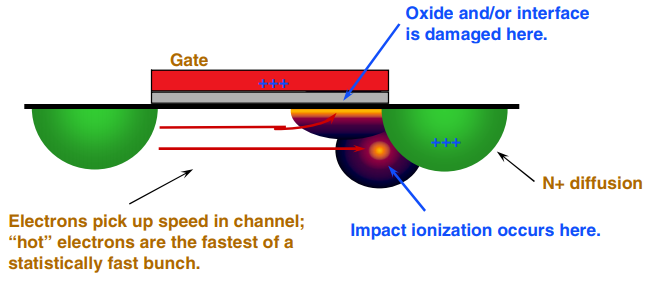
\includegraphics[width=0.7\textwidth]{hot}
\end{center}
	\end{frame}
	\begin{frame}
		\frametitle{Analysis Output from Power Grid Analysis}
			\begin{center}
				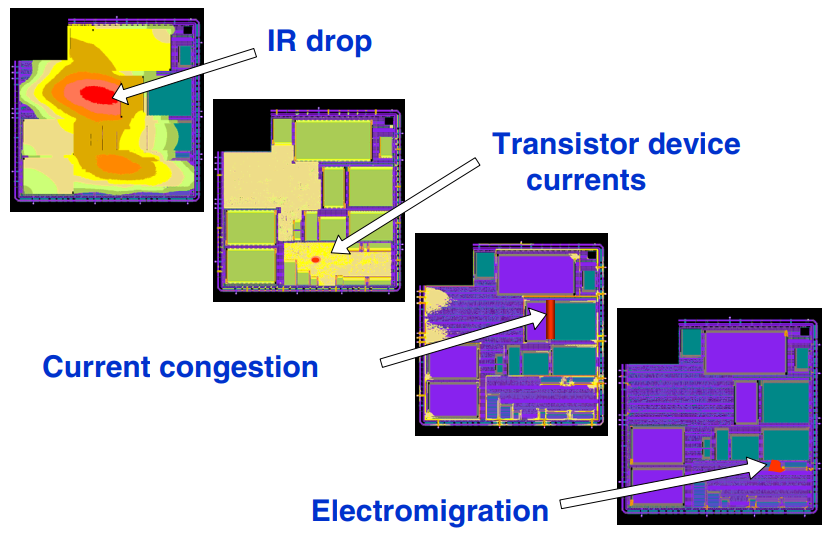
\includegraphics[width=\textwidth]{analysis}
			\end{center}
	\end{frame}
	%--------------------------------------------------	
	\begin{frame}
		\frametitle{Wrap up}
		\begin{center}
			\<بِسْمِ اللَّـهِ الرَّحْمَـٰنِ الرَّحِيمِ> \\
			\<وَمَا أُوتِيتُمْ مِنَ الْعِلْمِ إِلَّا قَلِيلً>
			
		\end{center}
	\end{frame}	
\end{document}